\section*{Time Series data}
Different sources
Price categories: Retail prices, wholesale prices

\subsection*{Wholesale prices}

\subsubsection*{Wholesale price index}
(taken from investopedia.com)\\
An index that measures and tracks the changes in price of goods in the stages before the retail level. Wholesale price indexes (WPIs) report monthly to show the average price changes of goods sold in bulk, and they are a group of the indicators that follow growth in the economy.\par
Although some countries still use the WPIs as a measure of inflation, many countries, including the United States, use the producer price index (PPI) instead.\par

\subsection*{Price sequences}

\subsubsection*{Preprocessing}
load data from csv into pandas dataframe 

removing NAs


\subsection*{Other sources}
distribution \& production

exchange rate
crude oil


\section*{Social Media data}
Twitter

\subsection*{Historical tweets}

\subsubsection*{Approach 1: Fetching "historical" tweets through Twitter API}

Using the Twython package for python we are able to interface with the Twitter API. Our methodology (figure \ref{fig:methodology}) is to select the twitter accounts of a number of regional celebrities as starting points. These are likely to `followed' by large numbers of local users. In a first phase (TWEET\_COLLECTION.py.get\_followers()), from each of these sources we may extract a list of followers and filter by various characteristics. Once a substantial list has been constructed it must be merged (merge.py and remove\_intersection.py), we may proceed to download the tweet activity (up to the 3200 most recent tweets) of each of these users in a second phase (TWEET\_COLLECTION.py.get\_tweets()).

Despite recent updates allowing developers greater access, Twitter still imposes troublesome constraints on the number of requests per unit time window (15 minutes) and, consequently, the data collection rate. It is therefore necessary to: 1) optimise the use of each request; and 2) parallelise the data collection effort.

As far as optimisation is concerned, the \textbf{GET statuses/user\_timeline} call may be called 300 times per 15 minute time window with up to 200 tweets returned per request. This sets a hard upper bound of 60000 tweets per time window. This is why the filtering stage of the first phase is so crucial. Using the \textbf{GET followers/list} call (30 calls/time window), we may discard in advance the majority of twitter users with low numbers of tweets (often zero), so as to avoid burning the limited user timeline requests on fruitless users, thus increasing the data collection rate. With this approach we may approach optimality and achieve 4-5 million tweets daily per process. However, it may be prudent to strike a balance between tweets per day and tweets per user. Therefore a nominal filter is currently set to 50 tweets minimum rather than 200. It is furthermore necessary to install dynamic time-tracking mechanisms within the source code so as to monitor the request rates and to impose a process 'sleep' when required.

Parallelisation begins with obtaining N ($\approx 10$) sets of developer credentials from Twitter (https://dev.twitter.com/). These N credentials may then be used to launch N processes (get\_users.sh) collecting user data in parallel. Given the decision to divide the follower collection and tweet collection into separate phases (this may alternatively be done simultaneously), there is no need for distributed interaction between the processes to control overlap, as each process will simply take $1/N$ th of the follower list produced in phase 1 and process it accordingly. It should be relatively simple to initiate this parallel computation given the design of the scripts.

\begin{table}
\begin{center}
\begin{tabular}{ | c | c | c | c | c | }
\hline
Phase 1  \\ \hline
Users & Duration (s) & Sleep (s) & User Rate & Type \\ \hline
334 & 2795 & 2047 & - & Total \\ \hline	    
299 & 2700 & 2047 & 99.7 & Normalised (3 windows) \\ \hline
Phase 2 \\ \hline
Tweets (Users) & Duration (s) & Sleep (s) & Tweet Rate & Type \\ \hline
171990 (334) & 3108 & 922 & - & Total \\ \hline
150008 (309) & 2700 & 922 & 50002.7 &  Normalised (3 windows) \\ \hline
\end{tabular}
\end{center}
\caption{A picture of the same gull looking the other way!}
\label{table:benchmark}
\end{table}

A benchmarking test (table \ref{table:benchmark}) performed in order to support configuration choices for the parallelisation. The test involved collecting the tweets from all good users within the first 20000 followers of @KareenaOnline, the account of a local celebrity. The following observations can be made:

\begin{itemize}
\item only 1.5-2\% of users are considered "good" under the current choice of filters (location, min. 50 tweets etc.);
\item Despite different levels of sleeping, phase 2 reads from users at roughly the same rate that phase 1 collects them (approximately 100 per time window in both cases);
\item Phase 2 produces around 50000 tweets per time window.
\end{itemize}

It is important to note however, that the rate of "good" users increases varies depending on the notoriety of the source account outside of India. To ensure good coverage for user collection, a wide variety of source users was chosen including rival politicians, musicians, sportspersons, film stars, journalists and entrepreneurs.

Tweet collection for Humanitas occurred in two main waves. In the first wave 180 000 users identifiers were collected. This amounted to 110 million tweets, collected over about three days, totalling 288GB of information (note a tweet response comprises the textual content as well as a substantial amount of meta data). In second wave of collection we encountered the effect of diminishing returns as many of the newly harvested users had already featured in the first wave. Despite a lengthier collection effort, only 110 000 new users were collected, leading to 70 million additional tweets and a grand total for the two waves of about 500GB of data. Future collection work for Humanitas would benefit from a more sophisticated approach, for example, by constructing a Twitter user graph.

\begin{figure}
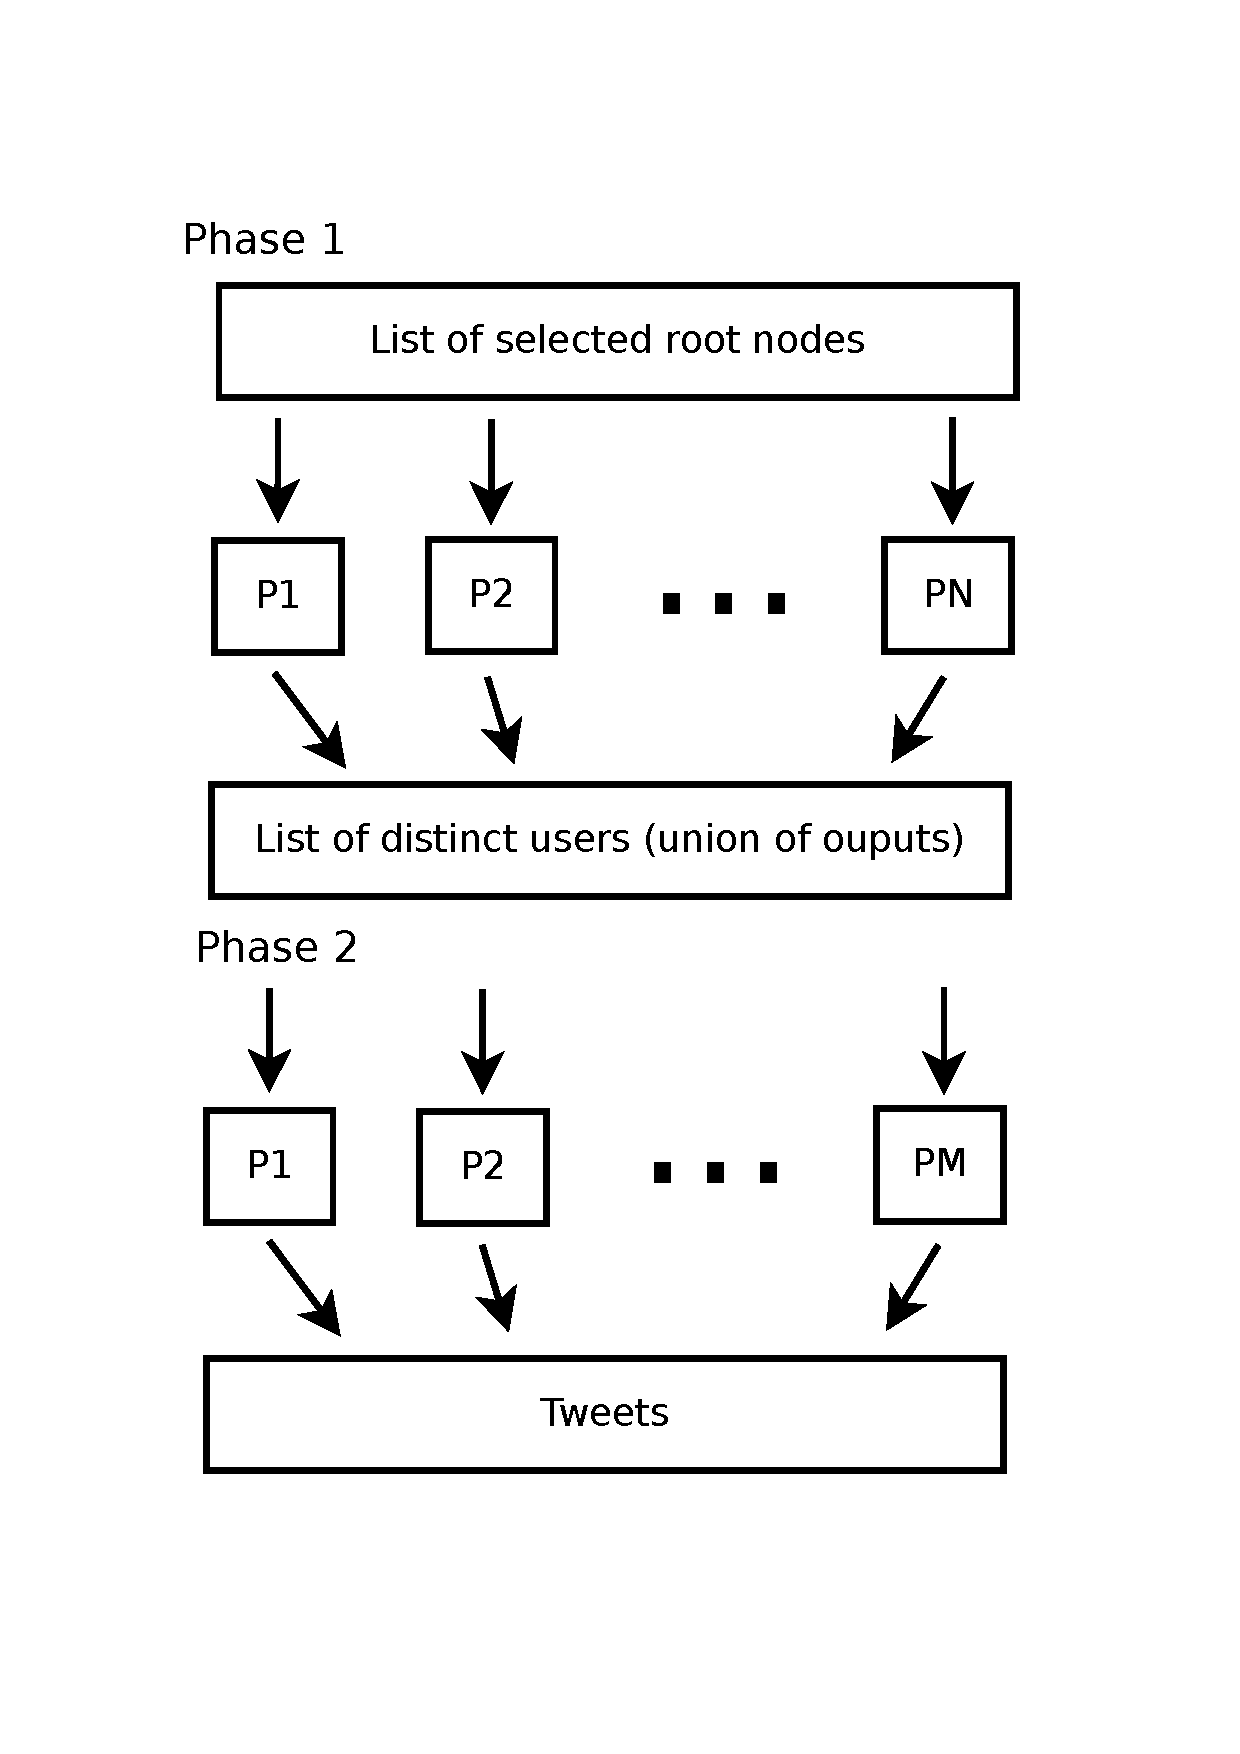
\includegraphics[width=.7\textwidth]{./img/CollectionProcess.pdf}
\caption{Tweet collection methodology.}
\label{fig:methodology}
\end{figure}

\subsubsection*{Approach 2: Filtering tweets provided by webarchive.org}
https://archive.org/details/twitterstream

\subsection*{Daily? tweet aggregator}

\subsubsection*{Clustering according to keywords}

\subsection*{Issue of localization}

\subsubsection*{Geolocalized tweets}
Filtering the available archives of tweets taken from the API yielded near to no geolocalized tweets from India matching our set of keywords. This reason is evident, because the twitter API only allows extraction of 1\% of tweets and only 2\% of tweets are actually geolocalized. In effect, getting tweets that match our keywords specific to food commodities is very unlikely. We had more luck with tweets from Indonesia, however as already explained we were unable to attain enough price sequences from Indonesia to actually train a model. Furthermore, the time constraints didn't allow us to get tweets from India and Indonesia in parallel in order to do some "stand-alone" clustering analysis.

\subsubsection*{Approximation: Mapping tweets to user location}


\section*{Processing}

\subsection*{Merging Series}

\subsection*{Crafting indicators from tweets}